
本节中,我们将概述Clang的结构和组织架构。将简要介绍一些重要的组件或子系统,然后在本书的后面部分会有专门的章节来进行进一步的扩展。我们希望这将让您对Clang的内部结构有一些了解,以及它们如何在读者自己的项目进行使用。

首先,来鸟瞰一下结构。下图显示了Clang的高层结构:

\hspace*{\fill} \\ %插入空行
\begin{center}
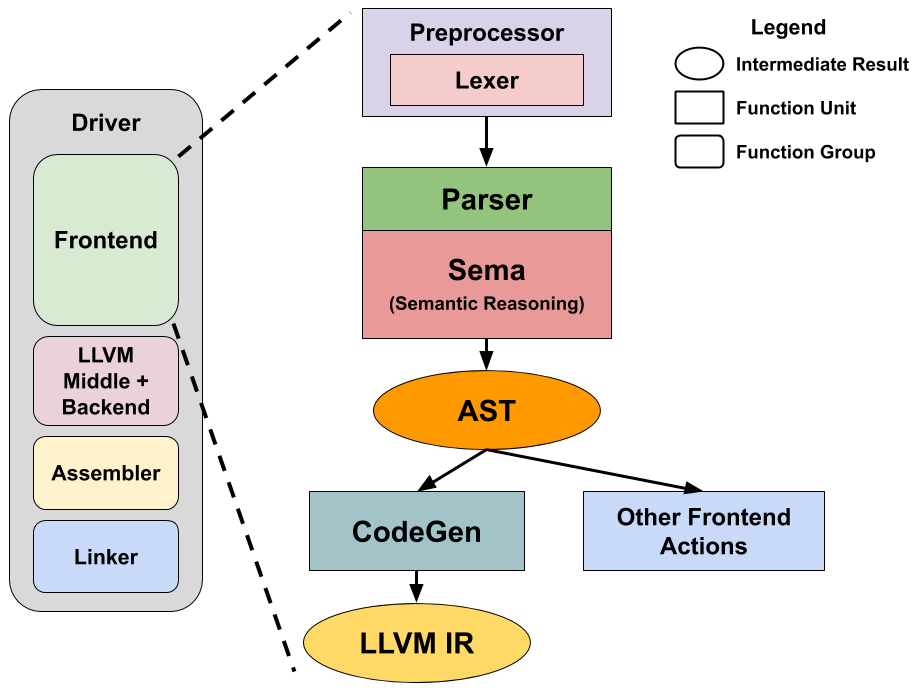
\includegraphics[width=0.7\textwidth]{content/2/chapter5/images/1.png}\\
图5.1 – Clang的高层结构
\end{center}

如图例中所示,圆角矩形表示由多个具有类似功能的组件组成的子系统,例如:前端可以进一步分解为一些组件,如预处理器、解析器和代码生成逻辑等。此外,还有中间结果,在前面的图表中显示为椭圆。我们对其中两个特别感兴趣——\textbf{Clang AST}和前者将在第7章中进行深入讨论,而后者则是本书第3部分“中端开发”的主要内容,会讨论可以应用于于LLVM IR的优化和分析。

让我们先看一下驱动程序的概述。下面的小节将简要介绍这些驱动程序组件。

\subsubsubsection{5.2.1\hspace{0.2cm}驱动}

常见的误解是,可执行文件\texttt{clang}是编译器的前端。虽然\texttt{clang}使用了Clang的前端组件,但可执行文件就是\textbf{编译器驱动},或者简称为\textbf{驱动}。

编译源代码是一个复杂的过程。首先,它由多个阶段组成,包括以下几个阶段:

\begin{itemize}
\item \textbf{前端}:解析和语义检查
\item \textbf{中端}:程序分析和优化
\item \textbf{后端}:原生代码生成
\item \textbf{汇编}:运行汇编器
\item \textbf{链接}:运行链接器
\end{itemize}

这些阶段及其包含的组件中,有无数的选项/参数和标志,例如:告诉编译器在哪里搜索包含文件的选项(即GCC和Clang中的\texttt{-I})。此外,我们希望编译器能够计算出一些选项的值,例如:编译器可以在头文件搜索路径中默认包含一些C/C++标准库的文件夹(例如,Linux系统中的\texttt{/include}和\texttt{/usr/include}),这样就不需要手动指定。继续这个例子,我们希望编译器能够跨不同的操作系统和平台进行移植,但是许多操作系统使用不同的C/C++标准库路径。那么,编译器如何能够正确的选择路径呢?

这种情况下,需要驱动来协助编译器。驱动充当核心编译器组件的管家,为它们提供必要的信息(例如,一个特定于操作系统的头文件包含路径),以便用户只需要提供重要的命令行参数即可。观察驱动程序的方法是在正常使用\texttt{clang}时添加\texttt{-\#\#\#}命令行标志。例如,可以尝试用这个标志编译一个简单的hello world程序:

\begin{tcblisting}{commandshell={}}
$ clang++ -### -std=c++11 -Wall ./hello_world.cpp -o hello_world
\end{tcblisting}

在macOS计算机上执行以上命令后,系统会显示如下信息:

\begin{tcblisting}{commandshell={}}
"/path/to/clang" "-cc1" "-triple" "x86_64-apple-macosx11.0.0"
"-Wdeprecated-objc-isa-usage" "-Werror=deprecated-objcisa-usage" 
"-Werror=implicit-function-declaration" "-emitobj" "-mrelax-all" 
"-disable-free" "-disable-llvm-verifier" … "-fno-strict-return" 
"-masm-verbose" "-munwind-tables"
"-target-sdk-version=11.0" … "-resource-dir"
"/Library/Developer/CommandLineTools/usr/lib/clang/12.0.0" "-isysroot"
"/Library/Developer/CommandLineTools/SDKs/MacOSX.sdk" "-I/usr/local/include" 
"-stdlib=libc++" … "-Wall" "-Wno-reorderinit-list"
\end{tcblisting}

\begin{tcblisting}{commandshell={}} "-Wno-implicit-int-float-
conversion" "-Wno-c99-designator" … "-std=c++11" "-fdeprecated-macro" 
"-fdebugcompilation-dir" "/Users/Rem" "-ferror-limit" "19" "-fmessage-length" 
"87" "-stack-protector" "1" "-fstackcheck" "-mdarwin-stkchk-strong-link" … 
"-fexceptions" … "-fdiagnostics-show-option" "-fcolor-diagnostics" "-o" 
"/path/to/temp/hello_world-dEadBeEf.o" "-x" "c++" "hello_world.cpp"…
\end{tcblisting}

这些信息,本质上是在驱动程序\textit{转译}之后传递给真正Clang前端的编译标志。虽然不需要理解所有这些标志的意思,但即使对于一个简单的程序,编译流程中也包含大量的编译器选项和许多子组件的使用。

驱动程序的源代码可以在\texttt{clang/lib/driver}下找到。在第8章中,我们将更仔细进行了解。

\subsubsubsection{5.2.2\hspace{0.2cm}前端}

编译器教科书可能会说,编译器前端由词法\textbf{分析器}和\textbf{解析器}组成,它们生成\textbf{抽象语法树(AST)}。Clang的前端也使用了这个结构,但有些不同。首先,分析器通常与\textbf{预处理器}耦合,对源代码执行的语义分析将分离到名为Sema的子系统中,这将构建一个AST,并执行所有类型的语义检查。

\hspace*{\fill} \\ %插入空行
\noindent
\textbf{分析器和预编译器}

由于编程语言标准的复杂性和实际源代码的规模,预处理变得非常重要,例如:当头文件层次结构有10层以上时,解析包含的文件就会变得棘手,这在大型项目中很常见。OpenMP会使用\texttt{\#pragma}来并行化循环,这使得像\texttt{\#pragma}这样的高级指令可能会受到挑战。如何解决这些挑战,就需要预处理器和分析器之间的合作,分析器可以为所有预处理操作提供原语,其源代码可以在\texttt{clang/lib/Lex}下找到。第6章中,我们将了解如何对预处理器和分析器进行开发,并学习如何使用强大的扩展系统实现自定义逻辑。

\hspace*{\fill} \\ %插入空行
\noindent
\textbf{解析器和Sema}

Clang的解析器使用来自预处理器和词法分析器的标记流,并试图实现其语义结构。在Sema子系统在生成AST之前,从解析器的结果获取更多的语义检查和分析相应的指令(变量名之类的标识符)。

Sema就是解析器完成的一个操作。后来人们发现这个额外的抽象层并不是必须的,所以解析器现在只与Sema交互。尽管如此,Sema仍然保留了这种回调风格的设计。例如,当解析for循环结构时,将调用\texttt{clang::Sema::ActOnForStmt(…)}函数(定义在\texttt{clang/lib/Sema/SemaStmt.cpp}中)。然后,Sema会做各种检查,以确保语法正确,并为for循环生成AST节点——这就是,\texttt{ForStmt}对象。

\hspace*{\fill} \\ %插入空行
\noindent
\textbf{AST}

当使用自定义逻辑扩展Clang时,AST是最重要的原语。我们将介绍的所有常用的Clang扩展/插件都是在AST上操作的。要体验AST,可以使用下面的命令(从源代码中)打印出一个AST:

\begin{tcblisting}{commandshell={}}
$ clang -Xclang -ast-dump -fsyntax-only foo.c
\end{tcblisting}

例如,在我的电脑上,我使用了以下简单的代码,只包含一个函数:

\begin{lstlisting}[style=styleCXX]
int foo(int c) { return c + 1; }
\end{lstlisting}

将产生以下输出:

\begin{tcblisting}{commandshell={}}
TranslationUnitDecl 0x560f3929f5a8 <<invalid sloc>> <invalid
sloc>
|…
`-FunctionDecl 0x560f392e1350 <./test.c:2:1, col:30> col:5 foo
'int (int)'
  |-ParmVarDecl 0x560f392e1280 <col:9, col:13> col:13 used c
'int'
  `-CompoundStmt 0x560f392e14c8 <col:16, col:30>
    `-ReturnStmt 0x560f392e14b8 <col:17, col:28>
      `-BinaryOperator 0x560f392e1498 <col:24, col:28> 'int' '+'
        |-ImplicitCastExpr 0x560f392e1480 <col:24> 'int' <LValueToRValue>
        |   `-DeclRefExpr 0x560f392e1440 <col:24> 'int' lvalue ParmVar 0x560f
              392e1280 'c' 'int'
        `-IntegerLiteral 0x560f392e1460 <col:28> 'int' 1
\end{tcblisting}

这个命令非常有用,因为C++ AST类代表特定的语言指令,这对于编写AST回调非常重要——而AST回调是许多Clang插件的核心。例如,从信息中可以知道变量的引用点(\texttt{c + 1}表达式中的\texttt{c})由\texttt{DeclRefExpr}类表示。

与解析器的组织方式类似,可以注册不同类型的ASTConsumer实例来访问或操作AST,稍后介绍的\textbf{CodeGen}就是其中之一。在第7章中,我们将展示如何使用插件实现自定义AST处理逻辑。

\hspace*{\fill} \\ %插入空行
\noindent
\textbf{CodeGen}

虽然没有规定应该如何处理AST(例如,使用\texttt{-ast-dump}命令行选项,前端将打印文本AST表示),但CodeGen子系统执行的最常见的任务是发出LLVM IR代码,稍后将由LLVM编译成原生程序集或目标代码。

\subsubsubsection{5.2.3\hspace{0.2cm}LLVM,组译器和连接器}

当CodeGen子系统产生LLVM IR代码,其将有LLVM编译管道进行处理,并生成原生代码,或是汇编代码,再或是目标代码。LLVM提供了一个称为\textbf{MC层}的框架,这个框架中体系结构可以选择实现直接集成到LLVM流水线中的汇编程序。主流架构,如x86和ARM都使用这种方法。如果不这样做,在LLVM管道末端发出的任何文本汇编代码,都需要由驱动程序调用外部汇编程序进行处理。

尽管LLVM有自己的链接器(即LLD),但集成的链接器仍不是一个成熟方案。因此,驱动程序总是调用外部链接器来链接目标文件,从而生成最终的二进制。

\begin{tcolorbox}[colback=blue!5!white,colframe=blue!75!black, fonttitle=\bfseries,title=外部与集成]
\hspace*{0.7cm}使用外部汇编程序或连接器意味着使用独立进程来运行程序。例如,要运行一个外部汇编程序,前端需要在启动汇编程序之前,将汇编代码放入一个临时文件,并将该文件路径作为命令行参数之一。另一方面,使用集成的汇编器/链接器会将汇编或链接的功能打包到库中,而不是打包到可执行文件中。因此,在编译管道的最后,LLVM将调用API来处理程序集代码在内存中的实例,从而产生目标代码。当然,这种集成方法的优点是可以节省许多间接的操作(写入临时文件,并立即读取它们),也会让代码在某种程度上更加简洁。
\end{tcolorbox}

至此,我们已经大致了解了从源代码到本机代码的普通编译流程。下一节中,我们将进阶对\texttt{clang}可执行文件的理解,并了解Clang提供的工具和扩展选项。这不仅增强了\texttt{clang}的功能,而且还提供了如何在LLVM之外的项目中,使用Clang的方法。





























